% Gerado automaticamente. No preambulo do documento use:
% \usepackage{pgfplots}
% \pgfplotsset{compat=1.18}
\definecolor{plotblue}{HTML}{2563EB}
\definecolor{plotorange}{HTML}{D97706}
\definecolor{plotgreen}{HTML}{059669}
\definecolor{plotpurple}{HTML}{7C3AED}
\definecolor{plotgray}{HTML}{374151}
\definecolor{plotred}{HTML}{DC2626}
\definecolor{plotteal}{HTML}{0F766E}
\definecolor{plotslate}{HTML}{64748B}

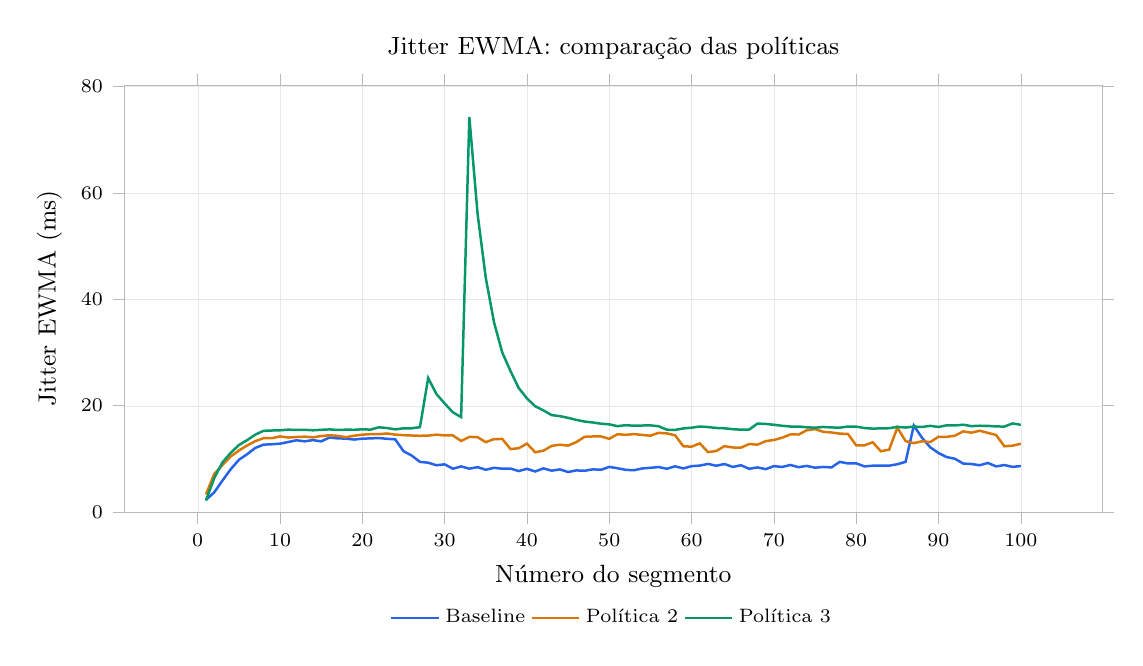
\begin{tikzpicture}
\begin{axis}[
    title={Jitter EWMA: comparação das políticas},
    xlabel={Número do segmento},
    ylabel={Jitter EWMA (ms)},
    width=14cm,
    height=7cm,
    grid=major,
    grid style={line width=.12pt, draw=gray!18},
    axis line style={draw=gray!55},
    tick style={draw=gray!55},
    tick align=outside,
    title style={font=\small},
    label style={font=\small},
    tick label style={font=\scriptsize},
    legend cell align={left},
    legend style={at={(0.5,-0.20)}, anchor=north, legend columns=3, draw=none, font=\scriptsize},
    ymin=0,
    ymax=80.2116
]
\addplot+[plotblue, line width=0.9pt, mark=none] coordinates {
(1,2.3)
(2,3.69)
(3,5.91)
(4,8.03)
(5,9.82)
(6,10.87)
(7,12.06)
(8,12.67)
(9,12.75)
(10,12.86)
(11,13.17)
(12,13.49)
(13,13.3)
(14,13.53)
(15,13.29)
(16,14.01)
(17,13.86)
(18,13.8)
(19,13.63)
(20,13.8)
(21,13.85)
(22,13.92)
(23,13.77)
(24,13.67)
(25,11.44)
(26,10.62)
(27,9.43)
(28,9.28)
(29,8.8)
(30,8.97)
(31,8.14)
(32,8.58)
(33,8.16)
(34,8.44)
(35,7.95)
(36,8.32)
(37,8.15)
(38,8.18)
(39,7.71)
(40,8.13)
(41,7.63)
(42,8.21)
(43,7.78)
(44,8.02)
(45,7.53)
(46,7.83)
(47,7.76)
(48,8.03)
(49,7.95)
(50,8.49)
(51,8.24)
(52,7.94)
(53,7.86)
(54,8.2)
(55,8.32)
(56,8.46)
(57,8.14)
(58,8.6)
(59,8.2)
(60,8.63)
(61,8.74)
(62,9.05)
(63,8.71)
(64,9.03)
(65,8.48)
(66,8.8)
(67,8.13)
(68,8.39)
(69,8.07)
(70,8.63)
(71,8.48)
(72,8.85)
(73,8.44)
(74,8.68)
(75,8.34)
(76,8.48)
(77,8.39)
(78,9.44)
(79,9.14)
(80,9.16)
(81,8.58)
(82,8.71)
(83,8.74)
(84,8.72)
(85,8.99)
(86,9.44)
(87,16.26)
(88,13.96)
(89,12.17)
(90,11.1)
(91,10.33)
(92,10.02)
(93,9.12)
(94,9.03)
(95,8.8)
(96,9.23)
(97,8.58)
(98,8.84)
(99,8.49)
(100,8.66)
};
\addlegendentry{Baseline}
\addplot+[plotorange, line width=0.9pt, mark=none] coordinates {
(1,3.31)
(2,7.14)
(3,8.83)
(4,10.44)
(5,11.57)
(6,12.51)
(7,13.33)
(8,13.9)
(9,13.88)
(10,14.22)
(11,14.01)
(12,14.11)
(13,14.17)
(14,14.05)
(15,14.29)
(16,14.44)
(17,14.33)
(18,14.07)
(19,14.36)
(20,14.55)
(21,14.65)
(22,14.65)
(23,14.77)
(24,14.56)
(25,14.46)
(26,14.39)
(27,14.34)
(28,14.37)
(29,14.55)
(30,14.41)
(31,14.41)
(32,13.36)
(33,14.13)
(34,14.08)
(35,13.14)
(36,13.72)
(37,13.74)
(38,11.85)
(39,12)
(40,12.87)
(41,11.24)
(42,11.54)
(43,12.44)
(44,12.66)
(45,12.5)
(46,13.15)
(47,14.15)
(48,14.21)
(49,14.22)
(50,13.77)
(51,14.64)
(52,14.52)
(53,14.66)
(54,14.5)
(55,14.36)
(56,14.9)
(57,14.79)
(58,14.43)
(59,12.37)
(60,12.29)
(61,12.92)
(62,11.27)
(63,11.48)
(64,12.39)
(65,12.14)
(66,12.11)
(67,12.79)
(68,12.67)
(69,13.33)
(70,13.55)
(71,13.98)
(72,14.59)
(73,14.58)
(74,15.38)
(75,15.59)
(76,15.09)
(77,14.96)
(78,14.75)
(79,14.68)
(80,12.55)
(81,12.54)
(82,13.13)
(83,11.43)
(84,11.73)
(85,15.88)
(86,13.35)
(87,12.95)
(88,13.32)
(89,13.16)
(90,14.16)
(91,14.14)
(92,14.36)
(93,15.17)
(94,14.92)
(95,15.29)
(96,14.88)
(97,14.49)
(98,12.37)
(99,12.48)
(100,12.85)
};
\addlegendentry{Política 2}
\addplot+[plotgreen, line width=0.9pt, mark=none] coordinates {
(1,2.15)
(2,6.36)
(3,9.33)
(4,11.12)
(5,12.6)
(6,13.52)
(7,14.56)
(8,15.27)
(9,15.33)
(10,15.37)
(11,15.49)
(12,15.44)
(13,15.46)
(14,15.37)
(15,15.46)
(16,15.54)
(17,15.43)
(18,15.49)
(19,15.47)
(20,15.56)
(21,15.5)
(22,15.93)
(23,15.8)
(24,15.54)
(25,15.75)
(26,15.75)
(27,15.96)
(28,25.19)
(29,22.19)
(30,20.42)
(31,18.75)
(32,17.86)
(33,74.27)
(34,56.08)
(35,43.99)
(36,35.67)
(37,30)
(38,26.51)
(39,23.32)
(40,21.37)
(41,19.9)
(42,19.11)
(43,18.23)
(44,18.03)
(45,17.71)
(46,17.33)
(47,17.01)
(48,16.84)
(49,16.61)
(50,16.49)
(51,16.15)
(52,16.33)
(53,16.23)
(54,16.27)
(55,16.3)
(56,16.13)
(57,15.48)
(58,15.45)
(59,15.72)
(60,15.86)
(61,16.08)
(62,15.98)
(63,15.81)
(64,15.75)
(65,15.58)
(66,15.48)
(67,15.51)
(68,16.63)
(69,16.57)
(70,16.41)
(71,16.22)
(72,16.08)
(73,16.08)
(74,15.94)
(75,15.86)
(76,16)
(77,15.91)
(78,15.86)
(79,16.08)
(80,16.06)
(81,15.8)
(82,15.69)
(83,15.73)
(84,15.76)
(85,16.01)
(86,15.89)
(87,16.07)
(88,16)
(89,16.21)
(90,16)
(91,16.31)
(92,16.28)
(93,16.42)
(94,16.16)
(95,16.23)
(96,16.2)
(97,16.1)
(98,16.07)
(99,16.66)
(100,16.4)
};
\addlegendentry{Política 3}
\end{axis}
\end{tikzpicture}
